
\documentclass[preprint,12pt]{elsarticle}

\usepackage[spanish]{babel}
\usepackage{amssymb}
\usepackage{graphicx}
\usepackage{lineno}
\usepackage[utf8]{inputenc}
\usepackage{url}

\journal{Journal Name}

\begin{document}
	
	\begin{frontmatter}
		
		
		\title{\huge Data Story Telling}
		
		\author{Balaguer Valles, Angela Lessly               (2016054494)}
		\author{Huallpa Castro, Leydi Katherine	      (2015053230)}
		\author{Pilco Quispe, Mireya Flavia		      (2015)}
		\author{Salamanca Contreras, Fiorella Rosmery (2015053237)}
		
		\address{Tacna, Perú}
		
		\begin{abstract}
			%% Text of abstract
			In this article an analysis is made of why Data Storytelling, or the stories we tell from the analysis of information, is important to make a program of analysis successful.

When talking to people who are successful in the subject of information analytics, usually, at some point, the phrase "tell a story with information" is mentioned. It seems obvious that no one doing a data analysis would like to create a narrative of the process and its results, but for many information analysts, this is not entirely obvious. So this article will explain the reasons why we believe that the information, and the stories created from the analysis of it, are so important.
	
		\end{abstract}
\end{frontmatter}
%%
	%% Start line numbering here if you want
	%%
	%\linenumbers
	
	%% main text
	\section{Resumen}
		En este artículo se hace un análisis de por qué el Data Storytelling, o las historias que contamos a partir del análisis de información, es importante para hacer que un programa de análisis sea exitoso. 

Cuando se habla con personas que tienen éxito en el tema de la analítica de la información, usualmente, en algún punto, se mencione la frase "contar una historia con la información". Pareciera obvio que nadie que esté haciendo un análisis de datos quisiera crear una narrativa del proceso y sus resultados, pero para muchos analistas de información, esto no es del todo obvio. Así que en este artículo se explicarán las razones por las cuales creemos que la información, y la historias creadas a partir del análisis de la misma, son tan importantes.\\

	%%
	%% Start line numbering here if you want
	%%
	%\linenumbers
	
	%% main text

\section{Objetivos}
		\begin{itemize}
		\item Objetivo 1: 
		\item Objetivo 2: 
		\item Objetivo 3: 
	\end{itemize}

	%%
	%% Start line numbering here if you want
	%%
	%\linenumbers
	
	%% main text

\section{Marco Teorico}
	\label{S:1}
\subsection{Data Storytelling}	

	El Data Storytelling es una herramienta que emplea la combinación de datos estadísticos y comunicación. Ayuda a las empresas a cumplir metas de comunicación y marketing contando mensajes de manera efectiva y cargados de información relevante para el público objetivo, también apoyados en instrumentos visuales y narrativos.\\
		
	\subsection{Elementos clave}
	
	El llamado Data Storytelling no es más que un enfoque estructurado sobre cómo comunicamos insights a partir de los datos, e involucra una combinación de tres elementos: datos, visualización y narrativa.
Ahora, ¿qué resulta de la combinación de estos elementos?, ¿cómo nos podemos beneficiar de ellos?, ¿necesitamos todos los elementos en cada análisis que hagamos?\\

			\begin{figure}[htb]
				\begin{center}
					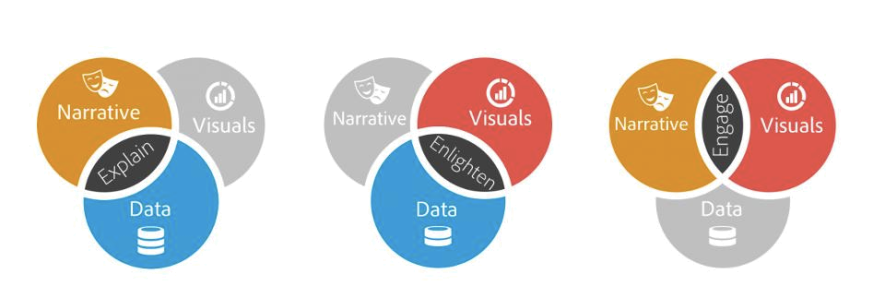
\includegraphics[width=18cm]{./Imagenes/img1}
				\end{center}
			\end{figure}
\begin{itemize}
		\item Narrativa + Datos = podremos explicar qué ha pasado y por qué un insight puede ser importante. Necesitaremos contexto para entender las 	conclusiones por completo.
		\item Visualización + Datos = Enlighten. Cuando añadimos una visualización a nuestros datos, podemos iluminar a nuestra audiencia con insights que no habrían visto de otra manera.
		\item Narrativa + Visualización = Engagement. La combinación perfecta para lograr ese interés e incluso para entretener a nuestra audiencia. 
	\end{itemize}

Pero, cuando unimos Visualización + Narración + Datos = Change, logramos contar una historia con nuestros datos, logramos influenciar y llevar a ese cambio que estábamos buscando.
\begin{figure}[htb]
				\begin{center}
					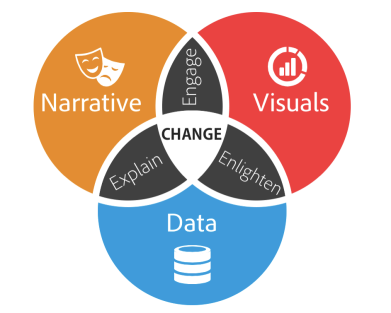
\includegraphics[width=10cm]{./Imagenes/img2}
				\end{center}
			\end{figure}
Y es que la pasión por los datos, ¡tiene que ir acompañada también por la pasión de contar historias! Si comunicas pobremente tus insights o si llegas a conclusiones erróneas, puede ser prácticamente peor que no utilizar ningún dato.

	\textbf{¿Por qué Data Storytelling?}

	\begin{itemize}
		\item Las historias son herramientas efectivas para transmitir la experiencia humana: esto ha sido así desde el inicio de los tiempos, pero ahora utilizamos datos y análisis para crear versiones mejoradas de esas historias. Gracias a ellas simplificamos y damos sentido a un mundo complejo.
		\item Para inspirar el cambio, necesitamos que entiendan nuestra historia: no importa cuántas horas hay detrás de nuestro análisis, no lograremos nada si no nos logramos explicar ya sea con una narrativa o con gráficos pero, necesitamos una historia.

		\item Las personas quieren evidencia del análisis que hay detrás: aunque nuestra audiencia no entienda el detalle de la analítica, sí quieren la evidencia de que hay datos detrás, ya que estas historias son más convincentes que solo una experiencia personal.

		\item Contar en una breve historia el resultado de horas de trabajo: se necesitan presentaciones cortas, con ideas concretas adaptadas a los stakeholders que recibirán la información para hacer llegar tu mensaje de una manera simple. 	
	\end{itemize}

	\subsection{Data Visualization}
	Es muy común que Data Storytelling se entienda solo como visualización de datos y, aunque como estamos viendo, es mucho más que eso, es cierto que la visualización es una parte esencial y muy potente como complementaria al análisis, para poder condensar grandes conjuntos de datos en una sola foto.\\
	
	\begin{itemize}
		\item Comprensión rápida de la información: gracias a las representaciones gráficas podemos ver grandes cantidades de datos de forma clara y coherente, lo que facilita la extracción de conclusiones e insights. Ganaremos tiempo y eficiencia para solucionar problemas.

		\item Identificar y actuar rápido sobre tendencias emergentes: incluso los archivos de datos casi infinitos, empiezan a tener sentido al representarse gráficamente; lo que nos permite detectar parámetros que están altamente correlacionados. Algunas relaciones serán obvias, pero otras tendremos que identificarlas para ayudar al cliente a enfocarse en ese punto de mejora que influenciará en sus objetivos principales.

		\item Identificar relaciones y patrones dentro de los activos digitales: descubrir tendencias dentro de los datos nos puede dar ventaja competitiva, como detectar puntos clave que están afectando a la calidad del producto o solucionar incidencias antes de que se conviertan en mayores problemas.

		\item Desarrollar un nuevo lenguaje de negocio para contar la historia a otros: una vez que hemos descubierto nuevos insights gracias a la analítica visual, el siguiente paso es comunicarlos, ya sea con gráficos simples o visualizaciones elaboradas, pero lo importante es lograr ese engagement y transmitir el mensaje rápidamente.	
	\end{itemize}
Para algunos, el esfuerzo de crear una historia alrededor de sus insights lo consideran innecesario y, además, una pérdida de tiempo. Pero creer que los datos deberían ser suficientes en sí mismos, solo porque sean explicados de una manera sencilla y concisa, para llevar a sus audiencias a tomar las decisiones necesarias, es lo mismo que creer erróneamente que las decisiones de negocio se toman teniendo en cuenta solo la lógica y la razón.\\


	\subsection{Pero, ¿qué nos permite?}
	El análisis de negocios depende de volúmenes suficientes de datos de alta calidad. La dificultad para garantizar la calidad de los datos es la integración y conciliación de los datos en diferentes sistemas, y luego decidir qué subconjuntos de datos estarán disponibles. \\

	%%
	%% Start line numbering here if you want
	%%
	%\linenumbers
	
	%% main text

\begin{LARGE}
		Ejemplo\\
	\end{LARGE}
	
	\begin{LARGE}
		Analisis\\
	\end{LARGE}
\newpage
\begin{LARGE}
		Conclusion\\
	\end{LARGE}
	
	\newpage
	
	\bibliographystyle{apalike} 	%ESTILO
	\bibliography{BIBLIOGRAFIA}		%ARCHIVO .bib
	
	%% The Appendices part is started with the command \appendix;
	%% appendix sections are then done as normal sections
	%% \appendix
	
	%% \section{}
	%% \label{}
	
	%% References
	%%
	%% Following citation commands can be used in the body text:
	%% Usage of \cite is as follows:
	%%   \cite{key}          ==>>  [#]
	%%   \cite[chap. 2]{key} ==>>  [#, chap. 2]
	%%   \citet{key}         ==>>  Author [#]
	
	%% References with bibTeX database:
	
	
	%% Authors are advised to submit their bibtex database files. They are
	%% requested to list a bibtex style file in the manuscript if they do
	%% not want to use model1-num-names.bst.
	
	%% References without bibTeX database:
	
	% \begin{thebibliography}{00}
	
	%% \bibitem must have the following form:
	%%   \bibitem{key}...
	%%
	
	% \bibitem{}
	
	% \end{thebibliography}
	
	
\end{document}

%%
%% End of file `elsarticle-template-1-num.tex'.
